\documentclass[10pt,a4paper]{report}
\usepackage[utf8]{inputenc}
\usepackage{amsmath}
\usepackage{amsfonts}
\usepackage{amssymb}
\usepackage{graphicx}
\author{Etaash Katiyar}
\title{FAR Work Trial}
\begin{document}

\section{Paper summary}
\subsection{Locating and Editing Factual Associations in GPT}
%- overall contributions
%- specific methodology
%- findings of locations
%- evaluation of results


Large language models (Transformer architectures) are able to store and produce facts.
 However, work is needed to determine understand how such facts are stored within the model. 
The paper presents a method to locate facts stored in a transformer language model, and understand the role of attention and intermediate MLPs in an LLM.\\
The method proceeds by computing three forward runs in the LLM,a clean run, a corrupted run, and a corrupted run with restoration of certain intermediate values.
The clean run proceeds on the unaltered transformer for a given input.
The corrupted run proceeds with significant random noise added to the initial embeddings of certain input tokens.
Intuitively, this corrupts the input embeddings.

The corrupted-with-restoration run computes a forward pass of the network with the corrupted initial embeddings, but fixes certain intermediate values to those computed in the clean run, and subsequent computation proceeds according to the transformer's weights unaltered.
The output distribution is compared between the corrupted run and the corrupted-with-restoration run, to get the indirect effect of an intervention.
The average indirect effect represents represents the contribution of intermediate values in the transformer to the output.
The indirect effect is averaged over a sample of facts.
The hidden state locations with largest average indirect effects are interpreted as the locations of facts stored in a large language model.
Further, the indirect effect of intervening on the intermediate attentions and MLP contributions are considered. 
[add a few sentences about the structure of the facts and which probabilities are considered]
 \\

It is found that there are distinctly two locations for facts, in the earlier layers of the transformer at the last subject token of the fact, and at the later transformer layers  at the last token of the input. 
Further, the earlier and later 'sites' decompose fairly cleanly into the indirect effects of the MLP contributions and the attention contributions, respectively.
These results are observed over a variety of large transformer models, as seen in the appendix of the paper.
\\
These observations are used to develop a technique to edit the facts stored in a transformer.
This method interesting on its own, but its efficacy also provides justification for the extracted fact locations. 
The MLP contributions are interpreted as linear associative memory, mapping input 'key' vectors to 'value vectors, and the edit method follows from this interpretation.
A new fact, represented by a new key value pair is formulated. The paper presents a method to formulate a new key value pair representing the new, edited fact.
The new key value pair is inserted into the network through an intuitive constrained optimization of weights of the intermediate MLP.
\\


\subsection{Experiment in extracting locations of sentiment}
% experimental setup
% graphs
% findings
% limitations

We propose an experiment to extract the location of sentiment in a transformer model, in a similar vein to the ROME paper. 

The transformer model (GPT-2) is used to classify sentiment. We append the text ' I am feeling' to the end of tweet text. Then, we run inference on the transformer and track the probabilities of the words 'good' and 'bad'.
Using a dataset of twitter tweets annotated with sentiment, we train a logistic regression classifier to predict the sentiment from these two probabilities. 
\\
Then, we use the output of the logistic regression as a proxy of the target we are interested in, namely the sentiment as predicted by the transformer. We then run clean inference, corrupted, and corrupted-with-patch runs of the transformer, and tracking the treatment effect on the sentiment proxy.
\\
Figures 1, 2, and 3 depict the effect of patching certain layers of the transformer on the proxy for sentiment. We observe an earlier and later site for the location. Further, these sites separate into attention and MLP effects as expected from the ROME paper. However, for longer inputs, the earlier site is not as distinct as in the ROME paper at the last input word of the subject.  

\begin{figure}[h]

\centering
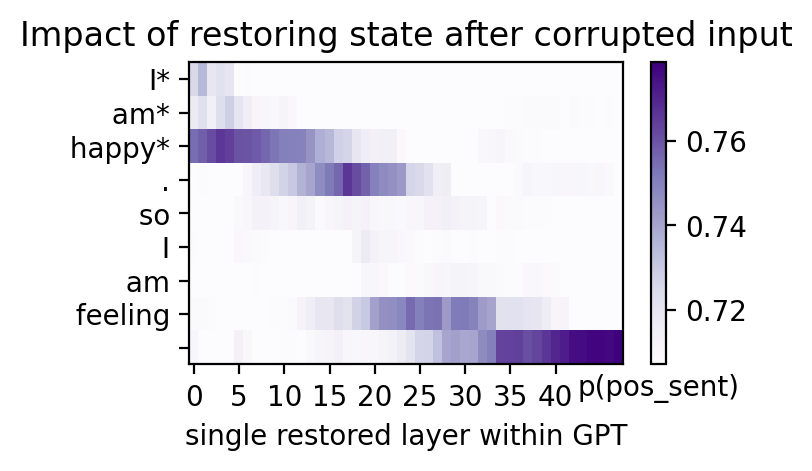
\includegraphics{toy_statement_trace1.png}
\caption{Toy statement causal trace}

\end{figure}

\begin{figure}[h]

\centering
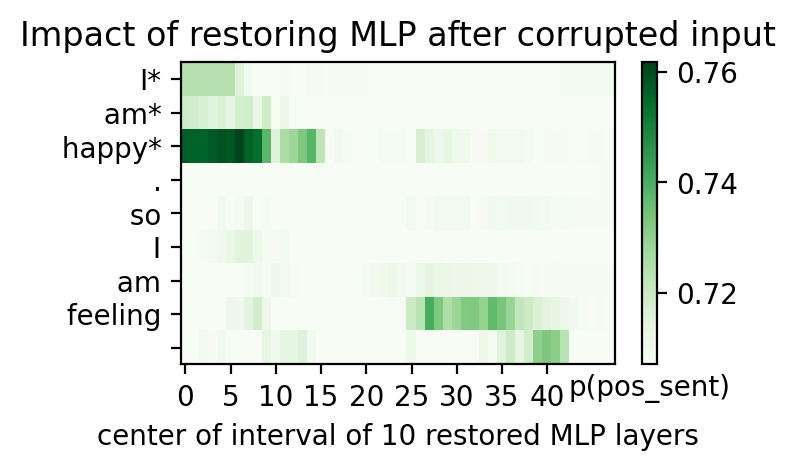
\includegraphics{toy_statement_trace2}
\caption{Toy statement causal trace (MLP}

\end{figure}


\begin{figure}[h]

\centering
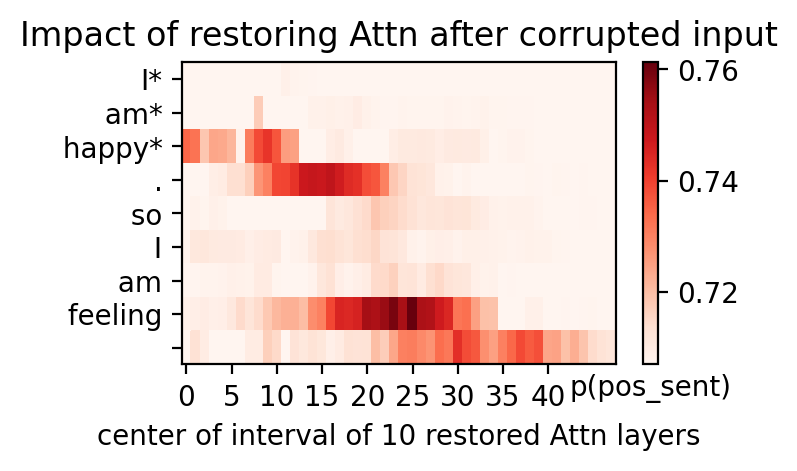
\includegraphics{toy_statement_trace3}
\caption{Toy statement causal trace (attn)}

\end{figure}

\textbf{Limitations}
More evidence is needed to determine how well this extracts the location of sentiment, and whether or not we are picking up certain erroneous artifacts. Attempting to edit the transformer's sentiment extraction could be useful for this purpose.
\\
Further, the proxy for sentiment is quite noisy, achieving only about 73\% accuracy. More work can be done to build a better proxy, perhaps by using the last hidden state of the transformer to predict sentiment. 
\\
Further, this method is quite slow for longer input sequences. 
\\

\end{document}